\documentclass{article}
\usepackage[utf8]{inputenc}
\usepackage{graphicx}
\usepackage{amsmath}
\usepackage{amssymb}

\title{Mat4 Aflevering 3}
\author{Roar Nind Steffensen}
\date{February 2016}

\begin{document}

\maketitle

\section*{Problem 2.15}
\begin{figure}[h!]
    \centering
    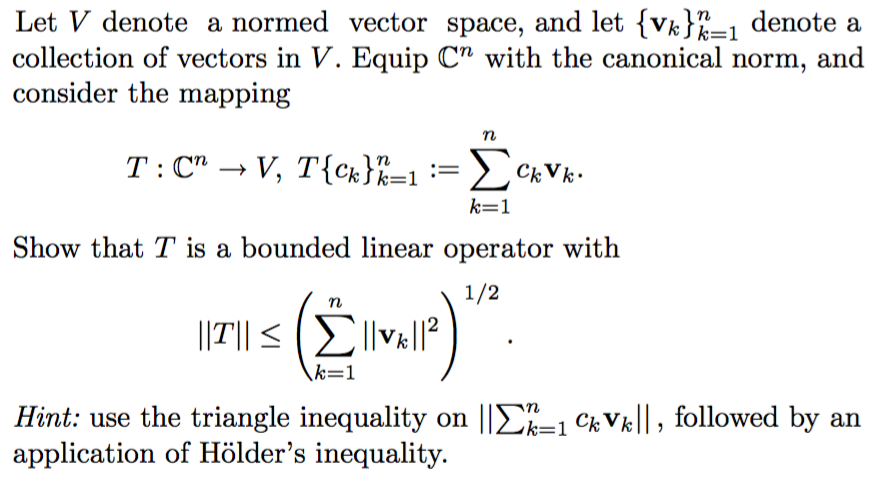
\includegraphics[width=\textwidth]{Fig/prob215}
\end{figure}
In order to use \textbf{definition 2.4.1} we need to show that the operator is linear using \textbf{equation (2.6) section 2.4}.
\begin{gather*}
    T (\alpha \{c_k\}_{k=1}^n + \beta \{y_k\}_{k=1}^n) = \sum_{k=1}^n \left(\alpha c_k + \beta y_k \right ) \mathbf{v}_k= \\
    \alpha\sum_{k=1}^n  c_k \mathbf{v}_k +\beta\sum_{k=1}^n  y_k \mathbf{v}_k = 
    \alpha T(\{c_k\}_{k=1}^n) + \beta T(\{y_k\}_{k=1}^n)  \\ \forall \; \alpha, \beta \in \mathbb{C}, \; \{c_k\},\{y_k\} \in V
\end{gather*}


Using \textbf{definition 2.4.1}, \textbf{the triangle inequality} and \textbf{Hölder's inequality}, we get

\begin{gather*}
 \text{ Inserting operator }\\ 
    \left|\left| T (\{c_k\}_{k=1}^n)\right|\right| = \left|\left| \sum_{k=1}^n c_k \mathbf{v}_k \right|\right|\\
\end{gather*}
\vspace{-1cm}
\begin{gather*}
     \text{ Using \textbf{the triangle inequality} } \\
    \left|\left| \sum_{k=1}^n c_k \mathbf{v}_k \right|\right| \leq  \sum_{k=1}^n \left|\left| c_k \mathbf{v}_k \right|\right| \\
\end{gather*}
\vspace{-1cm}
\begin{gather*}
    \text{ Using \textbf{Hölder's inequality} } \\
    \sum_{k=1}^n \left|\left| c_k \mathbf{v}_k \right|\right| \leq \left( \sum_{k=1}^n \left|\left| c_k \right|\right|^p \right)^{1/p} \left(\sum_{k=1}^n \left|\left| \mathbf{v}_k \right|\right|^q \right)^{1/q} 
\end{gather*}\\ 

Since we know that $\mathbb{C}^n$ is equipped with the canonical norm, and from \textbf{theorem 1.7.3 (Hölders inequality)} we know that $1/p+1/q=1$, we get that p and q must equal 2. Also the canonical norm on each element of a sum gives a absolute values of the elements, which transforms the sum into the canonical norm itself. Leaving us with: 

\begin{gather*}
    \left|\left| T (\{c_k\}_{k=1}^n)\right|\right| \leq K \left|\left| c_k \right|\right|_2
\end{gather*}
 With 
 \begin{gather*}
     K=\left(\sum_{k=1}^n \left|\left| \mathbf{v}_k \right|\right|^2 \right)^{1/2} 
 \end{gather*}
 Which is given to be $||T||$ in the assignment (meaning the minimum value for $K$). This shows that $T$ is a bounded linear operator with the given operator norm.
 
 
 
 
 
\section*{Problem 4.2}
\begin{figure}[h!]
    \centering
    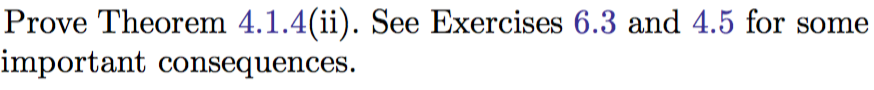
\includegraphics[width=\textwidth]{Fig/prob42}
\end{figure}

\textbf{Theorem 4.1.4 (ii)} states that 
\begin{gather*}
    ||v+w||^2+||v-w||^2=2\left(||v||^2+||w||^2 \right)
\end{gather*}

Which can be found using \textbf{definition 4.1.1} for spaces with an inner product and \textbf{lemma 4.1.3} combining the inner product with the norm of the vector space.

\begin{gather*}
\text{ Translating from norm squared to inner product } \\
    ||v+w||^2+||v-w||^2 = \langle v+w,v+w\rangle +\langle v-w,v-w\rangle 
\end{gather*}
\vspace{-0.5cm}
\begin{gather*}
    \text{Using \textbf{definition 4.1.1 (i)}} \\
    \langle v+w,v+w\rangle +\langle v-w,v-w\rangle = \\
    \langle v, v+w \rangle + \langle w,v+w \rangle + \langle v,v-w \rangle -\langle w,v-w \rangle
\end{gather*}
\vspace{-0.5cm}
\begin{gather*}
\text{ Using \textbf{definition 4.1.1 (ii)}} \\
\langle v, v+w \rangle + \langle w,v+w \rangle + \langle v,v-w \rangle -\langle w,v-w \rangle = \\ 
\overline{\langle v+w, v \rangle } + \overline{\langle v+w,w \rangle} + \overline{\langle v-w,v \rangle} - \overline{\langle v-w,w \rangle}  
\end{gather*}
\vspace{-0.5cm}
\begin{gather*}
\text{ Using \textbf{definition 4.1.1 (i)}} \\
\overline{\langle v+w, v \rangle } + \overline{\langle v+w,w \rangle} + \overline{\langle v-w,v \rangle} - \overline{\langle v-w,w \rangle}  = \\
\overline{\langle v,v \rangle} + \overline{ \langle w,v \rangle} + \overline{\langle v,w \rangle} + \overline{ \langle w,w \rangle} + \overline{\langle v,v \rangle} -\overline{ \langle w,v \rangle}-\overline{ \langle v,w \rangle} + \overline{ \langle w,w \rangle}
\end{gather*}\\

By reducing this, and using that $\langle v,v \rangle = \overline{ \langle v,v \rangle}$ we get
\begin{gather*}
    ||v+w||^2+||v-w||^2 = 2\left(||v||^2+||w||^2 \right) \: \square
\end{gather*}

\section*{Problem 4.5}
\begin{figure}[h!]
    \centering
    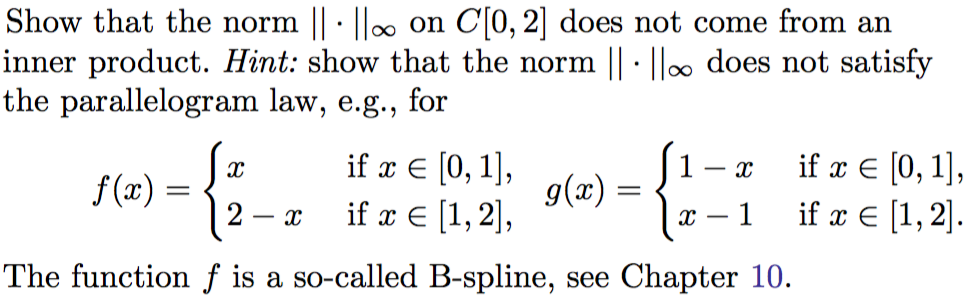
\includegraphics[width=\textwidth]{Fig/prob45}
\end{figure}

By looking at the lhs of \textbf{the parallelogram law}, we get 
\begin{gather*}
    ||f(x) + g(x)||_\infty^2 + ||f(x)-g(x)||_\infty^2
\end{gather*}
We first look at the absolute values of the terms.
\begin{gather*}
    |f(x) + g(x)|^2 + |f(x)-g(x)|^2
\end{gather*}
Which gives us the following values if we insert the functions
\begin{gather*}
    \left|_{2-x+x-1,\: \text{x $\in$ [1,2]}}^{x+1-x,\: \text{x $\in$ [0,1]}}\right|^2 + \left|_{2-x-x+1,\: \text{x $\in$ [1,2]}}^{x-1+x,\: \text{x $\in$ [0,1]}} \right|^2 \Rightarrow \\
    \left|1\right|^2 + \left|_{3-2x,\: \text{x $\in$ [1,2]}}^{2x-1,\: \text{x $\in$ [0,1]}} \right|^2
\end{gather*}

And if we look at the supremum norm again, and look at the highest possible value for a given value of x, we get

\begin{gather*}
    \left|1\right|^2 + \left|1\right|^2 = 2
\end{gather*}

Now we look at the rhs of \textbf{the parallelogram law}

\begin{gather*}
    2\left(||f||_\infty^2 + ||g||_\infty^2\right) = 2 ( |1|^2 + |1|^2 ) = 4
\end{gather*}

With the maximum (since it is a closed interval of continuouous functions, the supremum value is the maximum value) values for $f(x)$ and $g(x)$ found as
\begin{gather*}
   \left( \text{sup} \{|f(x)| \; | \; x \in [0,2]\} \right)^2 = |f(1)|^2 = |1|^2 \\
   \left( \text{sup} \{|g(x)| \; | \; x \in [0,2]\} \right)^2 = |g(0)|^2 = |g(2)|^2 = |1|^2
\end{gather*}

This leaves us with the contradiction saying $2=4$ which cannot be true, meaning that the supremum norm on $C[0,2]$ does not come from an inner product.


\end{document}
